\section{Pattern und Konzepte für Resilienz in verteilten Systemen}

%(der Hauptteil umfasst typischerweise ca. 2/3 bis 3/4 des Texts der Arbeit.)

\subsection{Circuit-Breaker}


Circuit-Breaker sind Entwurfsmuster, die dazu dienen, Fehler in verteilten Systemen zu isolieren,
indem sie den Zugriff auf fehlerhafte Dienste vorübergehend blockieren,
um eine Überlastung zu verhindern und die Systemstabilität zu gewährleisten.

\citet{Montesi.19.09.2016} heben die Rolle von Circuit-Breaker in Microservices-Architekturen hervor,
um kaskadierende Fehler zu vermeiden. % TODO "and" --> "und"
Microservices sind autonome Dienste, die über Message Passing kommunizieren, % Was ist Message Passing?
während bei \textit{Serviceorientierter Architektur} (SOA) die Komponenten einer Anwendung Teil eines
einzigen ausführbaren Artefakts, eines Monolithen, sind.

Die Hauptvorteile der \textit{Microservices-Architektur} (MSA) bestehen darin,
dass Komponenten unabhängig voneinander bereitgestellt und verwaltet werden können,
dass neue Versionen schrittweise eingeführt werden können, dass Komponenten
mithilfe verschiedener Technologien spezialisiert werden können und dass die Skalierung
effizienter durchgeführt werden kann.
Der hohe Verteilungsgrad der MSA bringt jedoch auch einige Herausforderungen mit sich,
wie z.B.\ Kommunikationsausfälle, die Überlastung von Diensten und die Notwendigkeit,
Änderungen an Dienst-APIs im Laufe der Zeit zu bewältigen.

Ein Ausfall in einer MSA gilt als unvermeidlich und kann
sich auf andere Dienste auswirken, die von dem ausgefallenen Dienst abhängig sind~\cite{Haley.28.06.2018,Montesi.19.09.2016}.
Es entsteht das Konzept des kaskadierenden Ausfalls, bei dem der Ausfall eines Dienstes
zu einem Dominoeffekt führen kann, der andere miteinander verbundene Dienste ebenfalls in
Mitleidenschaft zieht.
Um dieses Problem zu entschärfen, wird das Circuit-Breaker-Muster als Präventivmaßnahme eingeführt,
um Ausfälle innerhalb einer einzelnen Komponente einzudämmen und systemweite Ausfälle zu verhindern.
Der Grundgedanke hinter dem Circuit-Breaker-Pattern ist „Fail Fast“, d.h.\ sobald ein Dienst Anzeichen % TODO Anführungszeichen
von Unreaktivität zeigt, sollten die Anrufer sofort aufhören, auf ihn zu warten,
und die Situation in der Annahme behandeln, dass der Dienst möglicherweise nicht verfügbar ist.

Circuit-Breaker spielen eine entscheidende Rolle bei der Verbesserung der Stabilität und
Belastbarkeit von Diensten innerhalb einer MSA\@.
Clients sind in der Lage, die Verschwendung von Ressourcen für nicht reagierende Dienste zu vermeiden,
indem sie Fehler schnell erkennen und ihre Aktionen entsprechend anpassen.
Gleichzeitig wird überlasteten Diensten die Möglichkeit gegeben, sich zu erholen,
indem sie laufende Aufgaben abschließen, ohne mit weiteren Anfragen bombardiert zu werden.
Die praktische Umsetzung eines Circuit Breakers beinhaltet die Überwachung der Ausfallraten von Anrufen,
die an einen bestimmten Dienst gerichtet sind.
Wenn der Dienst Leistungsprobleme wie langsame Antworten oder häufige Fehler aufweist,
wird der Circuit-Breaker-Mechanismus ausgelöst,
sodass zukünftige Aufrufe sofort eine Fehlerantwort zurückgeben.

Das Circuit-Breaker-Muster lässt sich als endliche Maschine mit verschiedenen Zuständen
und Übergängen darstellen, die durch eine Reihe von Parametern in einer Steuertabelle gesteuert werden.
Durch die Nutzung des Leistungsschaltermusters werden die Zuverlässigkeit der Dienste und die
Ausfallsicherheit des Systems in einer MSA-Umgebung erheblich verbessert.
Dieser proaktive Ansatz schützt nicht nur vor kaskadierenden Ausfällen,
sondern gewährleistet auch eine effiziente Ressourcennutzung und fördert den allgemeinen Zustand
der miteinander verbundenen Dienste.


\paragraph{Deployment}

In diesem Paper werden drei verschiedene Ansätze für die Implementierung von Circuit-Breaker
in einer MSA diskutiert.

Der Circuit-Breaker wird in der Regel innerhalb der \textbf{Clients} eingesetzt,
wo er Aufrufe an externe Dienste abfängt.
Diese Strategie verhindert, dass Nachrichten den Zieldienst erreichen, wenn der
Leistungsschalter geöffnet ist, wodurch die Notwendigkeit ähnlicher
Schutzmechanismen im Dienst entfällt.
Allerdings beruht dieser Ansatz auf der Annahme, dass Clients zur Verwendung der Circuit Breaker
gezwungen werden können und dass sie nicht böswillig sind.
Der Nachteil besteht darin, dass das Verfügbarkeitswissen eines Dienstes auf den Client beschränkt ist,
sodass regelmäßige Pings erforderlich sind, um den Dienstintegritätsstatus abzufragen.

Eine alternative Implementierungsstrategie besteht darin,
Circuit-Breaker auf der Seite der \textbf{Dienste} oder in \textbf{Proxys} zwischen Kunden und Diensten einzuführen.
Dieser Ansatz hat seine eigenen Vor- und Nachteile.
Wenn der Circuit-Breaker auf der Seite des Dienstes platziert ist,
kann er den Dienst davor schützen, durch fehlgeschlagene Anfragen von mehreren Clients überfordert zu werden.
Außerdem hat der dienstseitige Circuit-Breaker einen globalen Überblick über die Verfügbarkeit des Dienstes,
im Gegensatz zu den client-seitigen Circuit-Breaker, die einen lokalen Überblick
auf der Grundlage der Interaktionen einzelner Clients haben.

Die Platzierung von Circuit-Breaker in Proxys zwischen Clients und Diensten
kann einen Mittelweg darstellen,
bei dem der Proxy die Kommunikation zwischen Clients und Diensten überwachen und steuern kann.
Dieser Proxy enthält für jedes Client-Dienst-Paar einen separaten Circuit-Breaker, der Anfragen nur dann zulässt,
wenn sowohl der Client- als auch der Dienst-Circuit-Breaker geschlossen sind.
Dieser Ansatz hat den Vorteil, dass keine Änderungen am Client- oder Dienstcode erforderlich sind,
da der Proxy unabhängig konfiguriert werden kann.
Außerdem schützt er sowohl Clients als auch Dienste, indem er Dienste vor zu aggressiven Clients und Clients
vor fehlerhaften Diensten abschirmt.
Allerdings führt der Proxy zu einem potenziellen Engpass im Netzwerk,
der möglicherweise durch den Einsatz mehrerer Proxys behoben werden muss.

\citet{Montesi.19.09.2016} schlagen vor, dass praktische Anwendungen diese verschiedenen Einsatzstrategien
kombinieren sollten, um die besten Ergebnisse zu erzielen.
Durch die Verwendung einer Kombination aus clientseitigen, dienstseitigen und proxy-basierten Circuit-Breaker
kann die Anwendung von den Vorteilen jedes Ansatzes profitieren und ihre jeweiligen Nachteile abmildern.
Diese Flexibilität bei der Bereitstellung ermöglicht eine robustere und effektivere Implementierung von Circuit-Breaker,
die die allgemeine Ausfallsicherheit und Verfügbarkeit des Systems verbessern kann.

Insgesamt bieten die drei vorgestellten Ansätze unterschiedliche Kompromisse in Bezug auf die Komplexität der Implementierung,
die Ressourcennutzung und den Grad des Schutzes, der den Clients und Diensten geboten wird.

\paragraph{Implementation}


Eine der bekanntesten Implementierungen von Circuit-Breaker ist die Hystrix-Bibliothek für Java,
während die Python-Bibliothek \textit{pybreaker} eine ähnliche Funktionalität bietet.
\textit{Pybreaker} ist eine flexible und leichtgewichtige Bibliothek, die es ermöglicht,
Python-Code in eine Prozedur zu verpacken, die von einem Circuit-Breaker gesteuert wird.
Diese Bibliothek hilft, den Ausfall von abhängigen Diensten oder Komponenten durch Überlastung
oder Fehler zu vermeiden und unterstützt Funktionen wie Fehlerzählung,
Zustandsüberwachung und benutzerdefinierte Rückfallstrategien. % Quelle?
\textit{Pybreaker} unterstützt sowohl Client- als auch dienstseitige Circuit-Breaker.

\tikzset{cross/.style={cross out, draw=black,thick, minimum size=10*(#1-\pgflinewidth), inner sep=1pt, outer sep=1pt,
    color=red, minimum height = 0.4cm},
%default radius will be 1pt.
cross/.default={1pt}}
\begin{figure}
\pgfdeclarelayer{background}
\pgfdeclarelayer{foreground}
\pgfsetlayers{background,main,foreground}
% Define a few styles and constants
\tikzstyle{state} = [draw, rounded corners,
text centered, minimum height=3em, minimum width=4em]
\centering
\centering
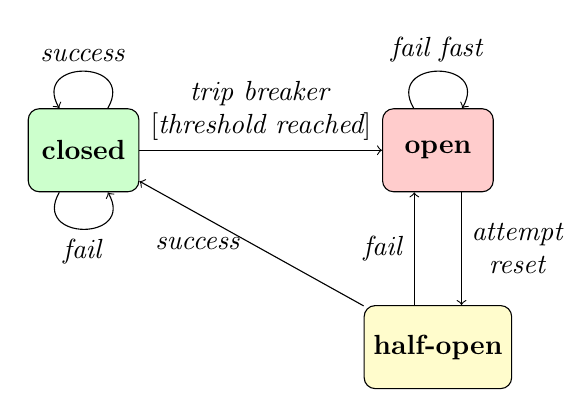
\begin{tikzpicture}[
%scale=0.6, every node/.style={scale=0.6}
]
\node (closed) [state, fill=green!20] {\textbf{closed}};
\node (open) [state, fill=red!20, right of=closed, node distance =4.5cm] {\textbf{open}};
\node (halfopen) [state, fill=yellow!20, below of=open, node distance =2.5cm] {\textbf{half-open}};
\draw [->] (closed) -- (open) node[above,midway,align=center] {\textit{trip breaker}\\\textit{$[$threshold
reached$]$}};
\draw [->] (halfopen) -- (closed) node[left,midway] {\textit{success}};
\draw [transform canvas={xshift=-0.3cm},->] (halfopen) -- (open) node[left,midway] {\textit{fail}};
\draw [transform canvas={xshift=0.3cm},->] (open) -- (halfopen) node[right,midway,align=center]
{\textit{attempt}\\\textit{reset}};
\path[]	(open)   edge[loop, in=60,out=120, looseness=3,->] node[above]  {\textit{fail fast}} (open);
\path[]	(closed)   edge[loop, in=60,out=120, looseness=3,<-] node[above]  {\textit{success}} (closed);
\path[]	(closed)   edge[loop, in=240,out=300, looseness=3,<-] node[below]  {\textit{fail}} (closed);
\end{tikzpicture}
\caption{Circuit Breaker Zustandsdiagramm nach~\cite{Montesi.19.09.2016}.}
\label{cb-fsm}
\Description{Circuit Breaker Zustandsdiagramm: closed/open/half-open}
\end{figure}

Je nach Zustand (geschlossen, offen oder halboffen) werden unterschiedliche
Aktionen ausgeführt, z.B.\ das Weiterleiten von Nachrichten, die
Behandlung von Fehlern oder das Blockieren von Anfragen, siehe Abbildung~\ref{cb-fsm}.

\subsection{Retry-Muster}

\textit{Retry} ist ein Architekturmuster, welches vorübergehende Fehler behandelt,
indem es fehlgeschlagene Operationen automatisch wiederholt, oft mit exponentiellen Backoff-Strategien.
Es eine bewährte Methode zur Verbesserung der Resilienz von Anwendungen,
die mit entfernten Diensten oder Netzressourcen kommunizieren~\cite{Meheden.2021}.
Wiederholungen sind ein entscheidender Aspekt für die Ausfallsicherheit von Anwendungen,
die in Containern oder in der Cloud ausgeführt werden~\cite{Haley.28.06.2018}.

\textit{Retry} ist eine effektive Technik zur Bewältigung vorübergehender Ausfälle in der
komponentenübergreifenden Kommunikation innerhalb eines Systems.
Azure und andere Cloud-Dienste und Client-SDKs bieten Wiederholungsfunktionalitäten, wie z.B.\ die Verwendung von
EnableRetryOnFailure von Entity Framework Core, um eine Wiederholungsstrategie für Datenbankaufrufe einzurichten~\cite{Haley.28.06.2018}.

% TODO Lesen: https://learn.microsoft.com/en-us/azure/architecture/patterns/retry

\paragraph{Bedingungen}

Für die Nutzung wird angenommen, dass die Fehlfunktion nur temporär ist.
Das Muster eignet sich besonders für Szenarien, in denen Fehler aufgrund von vorübergehender Nichtverfügbarkeit
oder Netzwerkkonnektivitätsproblemen auftreten~\cite{Meheden.2021}.

\begin{figure}[t]
    \centering
    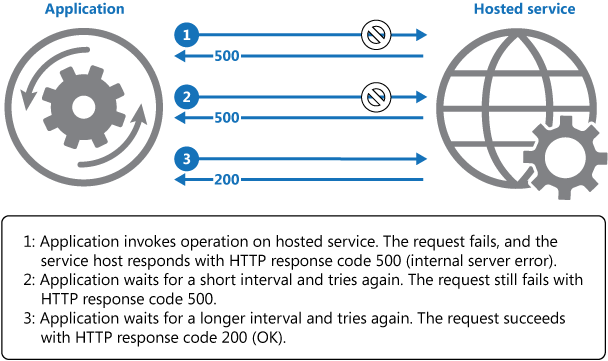
\includegraphics[width=\linewidth]{images/retry-pattern}
    \caption{Aufrufen eines Vorgangs in einem gehosteten Dienst unter Verwendung von \textit{Retry}~\cite{Microsoft.}}
    \label{fig:retry}
    \Description{Kommunikationsvorgang zwischen einer Anwendung und einem gehosteten Service, zwei Aufrufe schlagen mit Status 500 fehl, der dritte ist erfolgreich (200).}
\end{figure}

Das Beispiel in Abbildung~\ref{fig:retry} zeigt, dass bei einem fehlerhaften Aufruf einer Dienstoperation
(z.B.\ Code 500) die Anwendung zunächst wartet und es erneut versucht.
Sollte der Fehler weiterhin bestehen, wird die Wartezeit verlängert, und schließlich
kann die Anfrage erfolgreich abgeschlossen werden (z.B.\ Code 200).

Die Wiederholungsstrategie muss jedoch an die spezifischen Geschäftsanforderungen angepasst werden.
So sollten weniger kritische Anfragen eher schnell scheitern, um die Benutzererfahrung nicht zu beeinträchtigen,
während bei größeren Verzögerungen die Anzahl der Wiederholungen begrenzt werden sollte.
Für erfolgreiche Implementierungen müssen Fehler gründlich protokolliert und getestet werden,
um potenzielle Probleme frühzeitig zu erkennen und zu beheben~\cite{Meheden.2021}.

Insgesamt trägt das Wiederholungsmuster dazu bei, die Fehlertoleranz und Stabilität von Anwendungen zu erhöhen,
indem es vorübergehende Fehler effektiv adressiert und die Auswirkungen auf die Geschäftsprozesse minimiert.

Die Kombination von Retry mit dem Circuit Breaker-Pattern kann die Ausfallsicherheit weiter erhöhen,
indem die Wiederholungsversuche nach einer bestimmten Anzahl von Fehlern gestoppt werden,
sodass das System sich erholen und anders reagieren kann, z.B.\ auf einen zwischengespeicherten Wert zurückgreifen kann.
% See ResilientHttpClient in https://azure.microsoft.com/de-de/blog/using-the-retry-pattern-to-make-your-cloud-application-more-resilient/

\paragraph{Vorteile}


\subsection{Fallback-Strategien}


\subsection{Failover-Muster}
Eine weitere wichtige Methode, die sich in diesem Kontext bewährt hat, ist das
Failover-Muster. Dieses Konzept ist darauf ausgerichtet, die Kontinuität eines
Systems auch bei Störungen oder Ausfällen sicherzustellen, indem es eine
nahtlose Umschaltung auf alternative Ressourcen oder Backup-Komponenten
ermöglicht. Solche Mechanismen sind besonders in verteilten Systemen und bei
Diensten, die auf hohe Verfügbarkeit und Zuverlässigkeit angewiesen sind,
unverzichtbar. Das Failover-Muster implementiert eine Architektur, die in der Lage
ist, bei einem Ausfall der primären Komponente automatisch eine redundante
Komponente zu aktivieren, ohne dass die Endbenutzer von der Störung betroffen
sind.

Es gibt verschiedene Arten von Failover, die sich in ihrer Architektur und ihrem
Einsatzzweck unterscheiden. Das Active-Passive-Failover, bei dem eine aktive
Hauptkomponente von einer passiven Backup-Komponente unterstützt wird, wird
häufig für kosteneffiziente Implementierungen genutzt. Das Active-Active-Failover
hingegen betreibt mehrere aktive Komponenten gleichzeitig, was eine bessere
Lastverteilung und kürzere Umschaltzeiten ermöglicht. Darüber hinaus gibt es
Hot, Warm und Cold Failover. Während Hot Failover eine sofortige Umschaltung
ermöglicht, indem die Backup-Komponente ständig einsatzbereit ist, bieten Warm
und Cold Failover kostengünstigere Alternativen mit längeren Umschaltzeiten, da
die Backup-Komponenten nur teilweise oder gar nicht vorab initialisiert sind.

Zu den Vorteilen des Failover-Musters gehört vor allem die Erhöhung der
Systemverfügbarkeit. Durch die Fähigkeit, automatisch auf redundante
Komponenten umzuschalten, können Ausfallzeiten minimiert werden, was die
Benutzererfahrung erheblich verbessert. Gleichzeitig stärkt das Muster die
Resilienz eines Systems, da es auf potenzielle Ausfälle vorbereitet ist und deren
Auswirkungen abfedert. Es bietet außerdem Flexibilität, da es in verschiedenen Systemtypen eingesetzt werden kann, sowohl in stateless als auch in stateful
Anwendungen, wobei es sich an die spezifischen Anforderungen anpassen lässt.

Dennoch bringt das Failover-Muster auch einige Nachteile mit sich. Die Implementierung erfordert zusätzliche Ressourcen wie Hardware oder virtuelle
Maschinen, was die Kosten erhöht. Insbesondere bei Active-Active-Setups kann
die Synchronisation von Daten und Zuständen die Systemleistung belasten und
zusätzliche Komplexität verursachen. Zudem können unerwartete Fehler im
Failover-Prozess selbst auftreten, die die Ausfallzeit verlängern oder neue
Probleme verursachen. Daher ist es entscheidend, Failover-Mechanismen
regelmäßig zu testen und zu optimieren, um ihre Zuverlässigkeit sicherzustellen \cite{failover-patterns}.
\subsection{Load Balancing}
Load Balancing ist eine wichtige Strategie, um die Leistung und Resilienz verteilter Systeme erheblich zu steigern. Hierfür wird die anstehende Arbeitslast dynamisch auf verfügbare Server oder Ressourcen aufgeteilt.

\subsubsection{Übersicht}
Drei Komponenten spielen hier eine wichtige Rolle. Im Mittelpunkt dieses Verfahrens steht der Load Balancer, eine Software- oder Hardwarekomponente, welche serverseitig über mehrere Dienste verwaltet. Die zweite Komponente ist eine Gruppe von gleichartigen Service-Instanzen, welche die eigentliche Geschäftslogik beinhalten. Eingehende Anfragen werden zuerst den Load Balancer gestellt, welcher diese dann mithilfe einer geeigneten Strategie möglichst gerecht auf die Service-Instanzen aufteilt.

Zuletzt ist eine Komponente von Nöten, welche verfolgt, wie viele Service-Instanzen in der Konstellation vorhanden sind und in welchem Zustand sich diese befinden, also Service Discovery bewerkstelligt. Dies erfolgt hier Server-Side: Ein Client hat keine Kenntnis über den Aufbau, also Topologie, dieses Systems~\cite{schoner2017analyse}. Ob Load Balancing überhaupt Anwendung findet oder wie viele Ressourcen zur Verfügung stehen, wird nicht kommuniziert. Stattdessen geschieht jede externe Kommunikation nur mit dem Lastverteiler, welcher intern mithilfe der Registry ermittelt, welche Dienstknoten geeignet und bereit sind, die Anfrage entgegenzunehmen. Der Lastverteiler vermittelt nach Auswahl des Knotens schließlich zwischen dem Client und dem gewählten Service.

Load Balancing ist ebenso mit clientseitiger Service Discovery möglich. Hier existiert also kein zentraler Load Balancer, stattdessen ist der Client \textit{Registry-aware}~\cite{schoner2017analyse} und wählt selbstständig einen passenden Serviceknoten aus, er verhält sich also selbst wie ein Load Balancer. Da die eigentliche Lastverteilungsmethodik dennoch ähnlich zur serverseitigen Discovery erfolgt und diese Methode speziell angepasste Clientsoftware benötigt, wird sie im weiteren Verlauf nicht näher erläutert.

\begin{figure}[t]
  \centering
  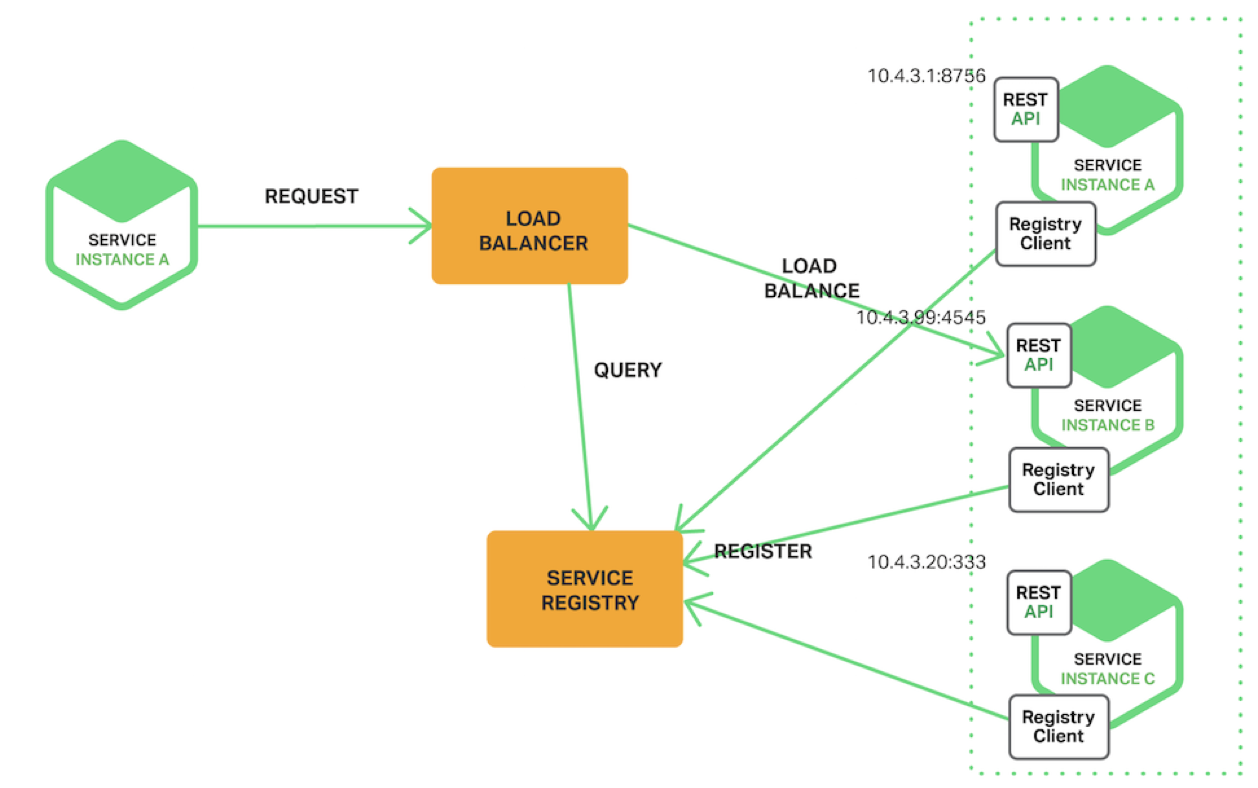
\includegraphics[width=\linewidth]{images/loadbalancer.png}
  \caption{Load Balancer mit drei Serviceinstanzen~\cite{schoner2017analyse}}
    \label{fig:loadbalancer}
  \Description{Load Balancer mit Serverseitiger Service Discovery und drei Serviceinstanzen}
\end{figure}

In Abb.~\ref{fig:loadbalancer} werden die drei Komponenten mit dem typischen Datenfluss schematisch dargestellt: die Dienstinstanzen registrieren sich bei ihrem Start in der Service Registry. Erfolgt nun eine externe Anfrage an den Load Balancer, fragt dieser wiederum die Registry an, welche Dienste angemeldet sind. Mit dieser Information kann ein Dienst ausgewählt werden, und die eigentliche Anfrageverarbeitung kann stattfinden. Die Anfrage (Abb.~\ref{fig:loadbalancer}, links) erfolgt nie direkt an eine der Dienstinstanzen.
\subsubsection{Zustandsverfolgung der Dienste}
Im vorherigen Beispiel verfolgt die Service Registry zuerst nur, ob ein Service gestartet wurde. Dafür registriert bzw. deregistriert sich der Service zum Start oder planmäßigen Ende seiner Ausführung.

Um eine effektive Lastverteilung zu ermöglichen reicht diese Information jedoch nicht aus. Wenn das Balancing ausschließlich realisiert wird, indem alle Anfragen \glq blind\grq{} auf Serviceknoten verteilt werden, könnten zwei Szenarien eintreten:
\begin{itemize}
	\item Obwohl die gleiche Anzahl an Anfragen fair an mehrere Knoten verteilt wird, könnte ein Knoten überlastet werden. Möglich wäre dies, wenn die entsprechenden Anfragen zufällig rechenintensiver sind als die Anfragen an andere Knoten. Ebenso denkbar ist, dass auf der Serverhardware andere Dienste oder (im Fall eines virtualisierten Computers) parallel ausgeführte virtuelle Maschinen mehr Rechenzeit verbrauchen (sogenannte \glqq Noisy Neighbours\grqq{}). Analog könnte eine langsamere Netzwerkanbindung zu unterschiedlichen Kapazitäten zwischen Knoten führen.
	\item Ein Serviceknoten könnte versagen. Beispielsweise könnte er ansprechbar sein, aber nur noch Fehlermeldungen zurückgeben. Alternativ antwortet er womöglich gar nicht mehr, oder benötigt derart viel Zeit, dass die Anfragen zum Zeitpunkt der Fertigstellung nicht mehr von Nutzen sind.
\end{itemize}

Es ist ersichtlich, dass ein pures Aufteilen der Anfragen auf die Serviceknoten ohne Einsicht in deren Zustände nicht sinnvoll ist. Aus diesem Grund wird die Service Registry erweitert um sogenannte \textit{Health Checks}: Jede Serviceinstanz kommuniziert ihre Auslastung und etwaige Fehler, und der Lastverteiler kann daraufhin sinnvolle Entscheidungen treffen.
%In beiden Fällen würde die Lastverteilung

\subsubsection{Strategien der Lastverteilung}\label{sec:loadbalancing-strats}
Die Auswahl eines Serviceknoten bei der Lastverteilung kann prinzipiell auf zwei Wege erfolgen. Bei der statischen Lastverteilung wird die aktuelle, tatsächliche Auslastung eines Knoten nicht beachtet, die Last wird stattdessen \glq blind\grq\ verteilt, und lediglich das Bereitsein der Knoten wird berücksichtigt~\cite{mishra.2020}. Beispiele statischer Strategien sind Round Robin, bei welcher anstehende Aufgaben zyklisch auf die Instanzen verteilt werden, oder das Load Balancing mit Hashing der Anfragen-IP-Adresse, bei welcher die Serviceknoten praktisch zufällig gewählt werden während mehrere Anfragen der gleichen Quelle immer auf dem gleichen Serviceknoten verarbeitet werden~\cite{g4g-loadbalancing}.
%\todo{im vergleich redundanz/partit./skal. bewerten}

Die dynamische Lastverteilung hingegen berücksichtigt die Momentanauslastung eines Serviceknotens. Gängige Strategien sind
\begin{itemize}
	\item Least Connection Load Balancing: Eine anstehende Aufgabe wird dem Dienst übergeben, welcher momentan die wenigsten aktiven Netzwerkverbindungen hat.
	\item Least Response Time Load Balancing: Die benötigte Zeit zur Vollendung der letzten Anfragen wird pro Serviceknoten protokolliert. Der Knoten, der historisch am schnellsten ist, erhält die nächste Aufgabe.
	\item Resource Based Load Balancing: Alle Serviceknoten berichten ihre aktuelle Auslastung anhand generischer Merkmale wie die CPU- oder Arbeitsspeicherauslastung. Dem Knoten mit der niedrigsten Auslastung wird die nächste Aufgabe zugewiesen.
\end{itemize}
















\subsection{DNS Round Robin}
Im vorherigen Abschnitt wurde eine Methode erläutert, mit der serverseitig mehrere Dienstinstanzen verwaltet und gebündelt und dann nach außen als eine Einheit kommuniziert werden. Dadurch steigt sowohl die Verfügbarkeit des Systems als auch die Kapazität für Anfragen, da mehrere Instanzen die gleiche Arbeit verrichten können und einzelne Ausfälle nicht zum Totalausfall führen.

Nichtsdestotrotz ist auch ein System mit Lastverteilung nicht ausfallsicher: der Lastverteiler selbst oder der gesamte Servercluster könnte ausfallen, woraufhin die Dienstleistung nicht mehr erreichbar wäre. Eine Strategie, um diesem Fall entgegenzusteuern, ist DNS Round Robin.

Das Domain Name System, kurz DNS, wird genutzt um eine Assoziation zwischen einem Hostname und einer IP-Adresse zu hinterlegen. Beispielsweise könnte ein Record hinterlegt werden, dass die Domain \verb|server.de| auf die Serveradresse des ersten Lastverteilers zeigt. Wenn ein Client nun anstelle einer IP-Adresse den zugehörigen Hostname benutzt, wird zuerst der lokale DNS (Cache) befragt, ob der Name zu einer IP aufgelöst werden kann. Ansonsten wird der externe autoritative Namensserver nach der IP befragt, und diese dann lokal zwischengespeichert und genutzt~\cite{Kopparapu.2002}.

Falls die IP des Lastverteilers nicht erreichbar ist, würde die Anfrage also fehlschlagen. Es ist jedoch möglich, für einen Hostname mehrere IP-Adressen zu hinterlegen. Diese würden dann zu verschiedenen Servercomputern, ggf. mit jeweils eigenen internen Lastverteilern führen.

Wenn ein Client nun zur Namensauflösung den autoritativen DNS befragt, gibt dieser immer alle Records zurück. Die Reihenfolge der IP-Adressen wird jedoch im Round Robin Verfahren zyklisch rotiert: wenn die erste Anfrage die drei Adressen \colorbox{lightgray}{A-B-C} erhält, würde die zweite Anfrage die Antwort \colorbox{lightgray}{B-C-A} erhalten.

So ist bereits für eine rudimentäre Lastverteilung gesorgt, da bei jeder Auflösung eine andere Adressreihenfolge herausgegeben und genutzt wird. Auch die Verfügbarkeit ist erhöht, da ein Client bei Nichterreichbarkeit einer Adresse zur Nächsten zurückgreifen kann.

\subsubsection{Vorteile}
DNS Round Robin hat zwei große Vorteile:
\begin{itemize}
	\item Es ist simpel zu implementieren, da keine spezielle Software auf dem Server- oder Clientsystem notwendig ist. Die Lastverteilung und Redundanz wird hier allein durch den Namensserver ermöglicht.
	\item Es schützt vor kompletter Nichterreichbarkeit. Ein Lastverteiler auf dem Server hilft nicht mehr wenn er selbst ausgefallen ist, oder wenn durch andere Probleme wie Geoblocks oder Firewalls gewisse IP-Ranges für den Client nicht erreichbar sind.
\end{itemize}

\subsubsection{Nachteile}
Auf den ersten Blick scheint dieses Verfahren ähnlich effektiv zu sein wie die statische Round Robin Lastverteilung aus Abschnitt \ref{sec:loadbalancing-strats}: Anfragen werden ohne Einsicht in die Ressourcenverfügbarkeit möglichst fair auf Kapazitäten aufgeteilt. Dies funktioniert in der Praxis jedoch nur eingeschränkt, da DNS-Einträge zwischengespeichert werden. Die Lastverteilung erfolgt also nur in seltenen Abständen. Besonders wenn regulär nur eine kleine Anzahl von Clients mit jeweils hohen Rechenanforderungen auf das System zugreifen, kann schnell durch Zufall eine ungleiche Auslastung entstehen (eine große Nutzerzahl würde erhebliche Schwankungen eindämmen).

Dieses Problem kommt erneut ins Spiel, wenn einer Überlastung entgegengesteuert werden soll. Nur neue Nutzer würden einen neu hinzugefügten DNS-Eintrag unmittelbar erhalten, wodurch eine erhebliche Verzögerung bis zur gleichverteilten Benutzung aller DNS-Einträge erfolgt.

Zuletzt ist auch das Verhalten im Fehlerfall nachteilhaft. Zwei Probleme haben den Ursprung darin, dass der Client die Verantwortung für das Failover-Verhalten übernimmt:
\begin{itemize}
	\item Der Rückfall auf die weiteren IP-Adressen kann nur erfolgen, wenn der Client einen Fehler bei dem Abruf der Primäradresse erkennt. Dies funktioniert wenn der Server nicht erreichbar ist. Wenn aber stattdessen beispielsweise Fehlercodes anstatt von Inhalt zurückgegeben werden, ist die Kommunikation mit dem Host aus Sicht des Clients erfolgt; es erfolgt kein Failover.
	\item Der Client kann erst nach einer gewissen Wartezeit davon ausgehen, dass eine Adresse ungültig ist. So kann eine erhebliche Wartezeit entstehen, bis das Failover-Verhalten ausgelöst wird~\cite{so-dns-slow}.%\todo{n. d. schrott}








\end{itemize}


\subsection{Recap}

\begin{figure}[t]
  \centering
  \resizebox{.8\linewidth}{!}{
  	% generated by Plantuml 1.2025.0
\definecolor{plantucolor0000}{RGB}{0,0,0}
\definecolor{plantucolor0001}{RGB}{241,241,241}
\definecolor{plantucolor0002}{RGB}{24,24,24}
\begin{tikzpicture}[yscale=-1
,pstyle0/.style={color=black,line width=1.5pt}
,pstyle1/.style={color=plantucolor0002,fill=plantucolor0001,line width=0.5pt}
,pstyle2/.style={color=plantucolor0002,line width=1.0pt}
,pstyle3/.style={color=plantucolor0002,fill=plantucolor0002,line width=1.0pt}
]
\draw[pstyle0] (8.5pt,37pt) -- (44.54pt,37pt) arc(270:360:3.75pt)  -- (54.04pt,53pt) -- (333.5pt,53pt) arc(270:360:2.5pt)  -- (336pt,109.5pt) arc(0:90:2.5pt)  -- (8.5pt,112pt) arc(90:180:2.5pt)  -- (6pt,39.5pt) arc(180:270:2.5pt) ;
\draw[pstyle0] (6pt,53pt) -- (54.04pt,53pt);
\node at (10pt,39pt)[below right,color=black,inner sep=0]{\textbf{Clients}};
\draw[pstyle0] (56.5pt,156pt) -- (206.94pt,156pt) arc(270:360:3.75pt)  -- (216.44pt,172pt) -- (221.5pt,172pt) arc(270:360:2.5pt)  -- (224pt,228.5pt) arc(0:90:2.5pt)  -- (56.5pt,231pt) arc(90:180:2.5pt)  -- (54pt,158.5pt) arc(180:270:2.5pt) ;
\draw[pstyle0] (54pt,172pt) -- (216.44pt,172pt);
\node at (58pt,158pt)[below right,color=black,inner sep=0]{\textbf{PlaybackService API (public)}};
\draw[pstyle0] (15.5pt,275pt) -- (252.9pt,275pt) arc(270:360:3.75pt)  -- (262.4pt,291pt) -- (262.5pt,291pt) arc(270:360:2.5pt)  -- (265pt,347.5pt) arc(0:90:2.5pt)  -- (15.5pt,350pt) arc(90:180:2.5pt)  -- (13pt,277.5pt) arc(180:270:2.5pt) ;
\draw[pstyle0] (13pt,291pt) -- (262.4pt,291pt);
\node at (17pt,277pt)[below right,color=black,inner sep=0]{\textbf{ContentRecommendationService API (private)}};
\draw[pstyle1] (21.64pt,71pt) arc (180:270:5pt) -- (26.64pt,66pt) -- (71.36pt,66pt) arc (270:360:5pt) -- (76.36pt,71pt) -- (76.36pt,91pt) arc (0:90:5pt) -- (71.36pt,96pt) -- (26.64pt,96pt) arc (90:180:5pt) -- (21.64pt,91pt) -- cycle;
\node at (31.64pt,76pt)[below right,color=black,inner sep=0]{Client 1};
\draw[pstyle1] (111.64pt,71pt) arc (180:270:5pt) -- (116.64pt,66pt) -- (161.36pt,66pt) arc (270:360:5pt) -- (166.36pt,71pt) -- (166.36pt,91pt) arc (0:90:5pt) -- (161.36pt,96pt) -- (116.64pt,96pt) arc (90:180:5pt) -- (111.64pt,91pt) -- cycle;
\node at (121.64pt,76pt)[below right,color=black,inner sep=0]{Client 2};
\draw[pstyle1] (201.64pt,71pt) arc (180:270:5pt) -- (206.64pt,66pt) -- (251.36pt,66pt) arc (270:360:5pt) -- (256.36pt,71pt) -- (256.36pt,91pt) arc (0:90:5pt) -- (251.36pt,96pt) -- (206.64pt,96pt) arc (90:180:5pt) -- (201.64pt,91pt) -- cycle;
\node at (211.64pt,76pt)[below right,color=black,inner sep=0]{Client 3};
\draw[pstyle1] (291.83pt,71pt) arc (180:270:5pt) -- (296.83pt,66pt) -- (315.17pt,66pt) arc (270:360:5pt) -- (320.17pt,71pt) -- (320.17pt,91pt) arc (0:90:5pt) -- (315.17pt,96pt) -- (296.83pt,96pt) arc (90:180:5pt) -- (291.83pt,91pt) -- cycle;
\node at (301.83pt,76pt)[below right,color=black,inner sep=0]{...};
\draw[pstyle1] (70.09pt,190pt) arc (180:270:5pt) -- (75.09pt,185pt) -- (202.91pt,185pt) arc (270:360:5pt) -- (207.91pt,190pt) -- (207.91pt,210pt) arc (0:90:5pt) -- (202.91pt,215pt) -- (75.09pt,215pt) arc (90:180:5pt) -- (70.09pt,210pt) -- cycle;
\node at (80.09pt,195pt)[below right,color=black,inner sep=0]{PlaybackService (stateless)};
\draw[pstyle1] (34.54pt,309pt) arc (180:270:5pt) -- (39.54pt,304pt) -- (238.46pt,304pt) arc (270:360:5pt) -- (243.46pt,309pt) -- (243.46pt,329pt) arc (0:90:5pt) -- (238.46pt,334pt) -- (39.54pt,334pt) arc (90:180:5pt) -- (34.54pt,329pt) -- cycle;
\node at (44.54pt,314pt)[below right,color=black,inner sep=0]{ContentRecommendationService (stateless)};
\draw[pstyle2] (47.94pt,96.39pt) ..controls (47.7pt,108.8pt) and (49.03pt,126.76pt) .. (57pt,140pt) ..controls (68.85pt,159.68pt) and (84.8066pt,171.7534pt) .. (102.6766pt,181.6934pt);
\draw[pstyle3] (107.92pt,184.61pt) -- (101.9993pt,176.7395pt) -- (103.5505pt,182.1795pt) -- (98.1105pt,183.7307pt) -- (107.92pt,184.61pt) -- cycle;
\node at (58pt,129pt)[below right,color=black,inner sep=0]{Handle Request};
\draw[pstyle2] (137.81pt,96.49pt) ..controls (137.13pt,105.54pt) and (136.34pt,117.44pt) .. (136pt,128pt) ..controls (135.36pt,147.61pt) and (136.2152pt,164.2673pt) .. (137.3052pt,178.6073pt);
\draw[pstyle3] (137.76pt,184.59pt) -- (141.0664pt,175.3127pt) -- (137.381pt,179.6044pt) -- (133.0894pt,175.9191pt) -- (137.76pt,184.59pt) -- cycle;
\node at (137pt,129pt)[below right,color=black,inner sep=0]{Handle Request};
\draw[pstyle2] (226.93pt,96.36pt) ..controls (224.62pt,108.75pt) and (219.95pt,126.71pt) .. (211pt,140pt) ..controls (198.63pt,158.36pt) and (183.8606pt,170.6242pt) .. (168.1706pt,181.1642pt);
\draw[pstyle3] (163.19pt,184.51pt) -- (172.8913pt,182.8117pt) -- (167.3405pt,181.7219pt) -- (168.4303pt,176.171pt) -- (163.19pt,184.51pt) -- cycle;
\node at (218.34pt,129pt)[below right,color=black,inner sep=0]{Handle Request};
\draw[pstyle2] (139pt,215.35pt) ..controls (139pt,237.8pt) and (139pt,275.01pt) .. (139pt,297.54pt);
\draw[pstyle3] (139pt,303.54pt) -- (143pt,294.54pt) -- (139pt,298.54pt) -- (135pt,294.54pt) -- (139pt,303.54pt) -- cycle;
\node at (140pt,248pt)[below right,color=black,inner sep=0]{Handle Request};
\end{tikzpicture}

  }
  \caption{Beispielarchitektur eines Streamingdiensts ohne Resilienz}
    \label{fig:example-arch}
  \Description{Systemarchitektur mit vier Clients, einem zentralen PlaybackService und einer Content Recommendation APIt}
\end{figure}


		
Für eine resiliente Architektur gibt es ist nicht die eine \enquote{richtige} Strategie. Die Vor- und Nachteile mehrerer Strategien sollten in einem mehrschichtigen Aufbau kombiniert werden, um die Leistung und Verfügbarkeit zu maximieren.

Zur Demonstration der in diesem Dokument beschriebenen Resilienzstrategien wird ein Videostreaming-Dienst als Beispielsystem entworfen. Das System in Abbildung~\ref{fig:example-arch} besteht aus einem Hauptdienst für die Videowiedergabe und einer separaten Content Recommendation API, die dem Nutzer personalisierte Inhalte vorschlägt. Die Architektur setzt auf bewährte Patterns wie Circuit Breaker, Load Balancing und Round Robin DNS, um eine hohe Verfügbarkeit und Fehlertoleranz zu gewährleisten.

Um eine hohe Nutzerzufriedenheit zu garantieren, sollte die Vorschlagsfunktion hier möglichst immer verfügbar sein. Sowohl lange Wartezeiten als auch Fehler und komplette Ausfälle müssen möglichst vermieden werden. Zuerst kann hierfür ein Circuit Breaker implementiert werden. So werden Dienstinstanzen vom System getrennt, wenn diese in einen Fehlerhaften Zustand geraten. Folglich können Fehler in Dienstknoten früh erkannt werden, und Instanzen können sich nach Abtrennung vom System erholen.

Um bei einem Ausfall der bisher einzigen Dienstinstanz sinnvoll reagieren zu können, müssen im nächsten Schritt redundante Instanzen implementiert werden. Mithilfe eines Load Balancers könnte man mehrere Dienste nach außen hin als einen einzelnen darstellen. So entstehen mehrere Vorteile: 
\begin{itemize}
	\item Funktionierende Knoten können Anfragen annehmen, obwohl ein oder mehrere andere ausgefallen sind. Das System ist weiter verfügbar.
	\item Es können mehr Nutzer den Dienst benutzen, da die Last auf beliebig viele Dienste verteilt werden kann. Kommen mehr Nutzer hinzu, kann das System also horizontal skaliert werden.
	\item Mithilfe von Autoscaling kann zuletzt sichergestellt werden, dass immer die richtige Anzahl von Dienstinstanzen verfügbar ist. Das heißt, dass zu Stoßzeiten ausreichend Kazazitäten zur Verfügung stehen, während das System zu Ruhezeiten nicht überdimensioniert ist. So steigt die Leistung, während Kosten gespart werden können.
\end{itemize}

Ebenso erdenklich ist jedoch, dass durch einen schwerwiegenderen Fehler keine Dienstinstanz mehr verfügbar ist. Dies ist denkbar wenn der Load Balancer versagt, oder eine schwerwiegende Netzwerkstörung im Rechenzentrum vorliegt. Dieser Fehler ist nicht unmittelbar lösbar, dennoch kann man das System ausfallresilient machen, schließlich ist eine geminderte User Experience besser als gar keine. Hier wäre ein Fallback zu einer statischen Liste (anstelle einer persönlichen Content Recommendation-Liste) denkbar. So hat ein Nutzer dennoch Vorschläge auf der Startseite dieses Streamingdienstes, und der Betrieb des Fallbackdiensts benötigt erheblich weniger Ressourcen und hat weniger Fehlerpotential.

Zuletzt könnte dieser gesamte Servercluster fehlschlagen; die IP-Adresse ist nicht mehr erreichbar. Auch davor kann man sich schützen: Obwohl das DNS Round Robin Nachteile hat, die es unter anderem zu einem suboptimalen Load Balancer macht, ist es eine sinnvolle \textit{Last Defense}. So kann auch im unwahrscheinlichen Fall eines Totalausfalls die Verfügbarkeit des Dienstes erhalten werden. Um die Latenz der Verbindung zu reduzieren und somit die Geschwindigkeit der Anwendung weiter zu erhöhen, könnte hier zusätzlich ein Geolocation-basiertes DNS eingerichtet werden, um Nutzer zu möglichst nahgelegenen Servern zu leiten.

Durch diese Kombination von Circuit Breaker, Load Balancing, einer Fallback-Strategie und von DNS-basiertem Balancing wird das System robuster gegenüber Lastspitzen und Ausfällen. Dieses Beispiel zeigt, wie diese Patterns in einem modernen verteilten System angewendet werden können, um Fehlerresilienz und -toleranz und Skalierbarkeit zu maximieren.
